\documentclass[unicode,12pt,aspectratio=169, dvipdfmx]{beamer}
\usepackage{bxdpx-beamer}
\usetheme[progressbar=frametitle]{metropolis}
\renewcommand{\kanjifamilydefault}{\gtdefault}%既定をゴシック体に
\usepackage{bm}
% \usepackage{color}
%\usepackage{graphicx}


%Artificial Identification: A Novel Privacy Framework for Federated Learning Based on Blockchain
% タイトル、著者、日付の情報
\title{Artificial Identification: A Novel Privacy Framework for Federated Learning Based on Blockchain}
\author{竹本志恩}
\date{\today}
% \subtitle{latexで作成}
\date[]{\today}
\institute{INIAD}
\subject{輪読}
% \keywords{LaTeX2e,Beamer,Presentation}
\AtBeginSection[]{
    \frame{{目次}\tableofcontents[currentsection, hideallsubsections]} %目次スライド
}




\begin{document}
% タイトルスライド
    \frame{\maketitle}
    \section{1. はじめに}
    \begin{frame}{書誌情報}
        \begin{columns}
            \begin{column}{.8\linewidth}
                \begin{itemize}
                    \item 題名
                    \begin{itemize}
                        \item Artificial Identification: A Novel Privacy Framework for Federated Learning Based on Blockchain
                    \end{itemize}
                    
                    \item 発表日
                    \begin{itemize}
                        \item 01 February 2023
                    \end{itemize}

                    \item 著者
                    \begin{itemize}
                        \item Liwei Ouyang, Fei-Yue Wang, Yonglin Tian, Xiaofeng Jia, Hongwei Qi, and Ge Wang
                    \end{itemize}

                    % \item 会議名
                    \item 論文誌名
                    \begin{itemize}
                        \item IEEE TRANSACTIONS ON COMPUTATIONAL SOCIAL SYSTEMS, VOL. 10, NO. 6, DECEMBER 2023
                    \end{itemize}
                    % \item 会議: IEEE ICC 2024
                \end{itemize}          
            \end{column}
        \end{columns}
    \end{frame}

    \begin{frame}{どんな研究?}
        \begin{columns}
            \begin{column}{.8\linewidth}
                \begin{itemize}
                    \item ブロックチェーンを適用するFLについて
                    % \note{項目2について熱く語る}
                    \item プライバシーとセキュリティを従来より確保し
                    \item 運用に必要なコストを削減する
                    % \small {* Federated Learning, 連合学習}
                \end{itemize}          
            \end{column}
        \end{columns}
    \end{frame}

    % \section{2. 前提の共有}

    \begin{frame}{ブロックチェーン}
        \begin{columns}
            \begin{column}[T]{.7\linewidth}
                \begin{itemize}
                    \item 公正で安定した記録システム
                    \item 改ざんや障害発生に強い
                    \item 記録の複製を複数の参加者が保持する
                    \item ・参加者が脱落してもシステムは動く
                    \item ・取引記録が残る
                \end{itemize}
            \end{column}
            % \begin{column}[T]{.5\linewidth}
            %     \begin{itemize}
            %         \item 図を入れる
            %     \end{itemize}
            % \end{column}
        \end{columns}
    \end{frame}

    \begin{frame}{スマートコントラクト}
        \begin{columns}
            \begin{column}[T]{.7\linewidth}
                \begin{itemize}
                    \item 公正で安定した記録システム
                    \item ブロックチェーン上で
                    \item 事前に定めた内容で契約し,取引を実行
                    \item 条件を満たすと自動で実行
                    \item 不正や改ざんを防ぎ,効率的な取引を実現
                \end{itemize}
            \end{column}
            % \begin{column}[T]{.5\linewidth}
            %     \begin{itemize}
            %         \item 図を入れる
            %     \end{itemize}
            % \end{column}
        \end{columns}
    \end{frame}



    \section{2. 動機}
    \begin{frame}{背景}
        \begin{columns}
            \begin{column}[T]{.6\linewidth}
                \begin{itemize}
                    \item FLの課題
                    \begin{itemize}
                        \item データ送受信に関する攻撃の危険性
                        \item 信頼性の低いノードによる問題の発生
                    \end{itemize}
                    \item ブロックチェーンの役割
                    \begin{itemize}
                        \item 安全なブリッジ
                        \begin{itemize}
                            \item グローバルモデルのダウンロード
                            \item ローカルモデルのアップロード
                        \end{itemize}
                    \item インセンティブメカニズムによる参加意欲の向上
                    \end{itemize}
                    \item 従来手法はプライバシの保護が不完全
                    \item 二種のスマートコントラクトで改善
                \end{itemize}
            \end{column}
            % \begin{column}[T]{.5\linewidth}
            % \end{column}
        \end{columns}
    \end{frame}


    % \begin{frame}{Federated Learningとは}
    %     \begin{columns}
    %         \begin{column}[T]{.7\linewidth}
    %             \begin{itemize}
    %                 \item 連合学習, FL
    %                 \begin{itemize}
    %                     \item 分散的に学習する手法の一つ
    %                     \item 各サーバはデータを持ち,学習
    %                     \item 学習結果をあるサーバで集約
    %                     \item 統合,パラメータサーバが存在
    %                 \end{itemize}  
    %                 \item 大まかな流れ
    %                 \begin{itemize}
    %                     \item 統合サーバからモデルを配布
    %                     \item 各パラメータサーバはローカルデータで学習
    %                     \item モデルのパラメータを統合サーバで集約
    %                     \item モデルを更新し再配布
    %                     \item 一連の流れを繰り返す
    %                 \end{itemize}    
    %             \end{itemize}          
    %         \end{column}
    %         \begin{column}[T]{.5\linewidth}
    %                 \begin{center}
    %                     % \includegraphics[scale=0.3]{figures/fl.png}
    %                     \scriptsize{FLのイメージ}
    %                 \end{center}
    %         \end{column}
    %     \end{columns}
    % \end{frame}


    % \begin{frame}{課題}
    %     \begin{columns}
    %         \begin{column}[T]{.7\linewidth}
    %             \begin{itemize}
    %                 \item IoTデバイス(ID)から基地局(BS)へのデータ転送
    %                 \item 想定されるシナリオ
    %                 \begin{itemize}
    %                     \item 各BSはサーバとIDを所持
    %                     \item BSにIDからデータを送信
    %                     \item サーバの持つデータでモデルを学習
    %                 \end{itemize}
    %                 \item FLの精度
    %                 \begin{itemize}
    %                     \item サーバの持つデータの量と分布が影響
    %                     \item 量と分布は制約の下決めた伝送先に依存
    %                     \item IDからどのBSに送信するかが重要
    %                 \end{itemize}
    %                 \item 帯域幅制約下でFLの精度を向上
    %                     \begin{itemize}
    %                         \item 制約により送信先が限定
    %                         \item その中で最適なBSを決定
    %                     \end{itemize}
    %             \end{itemize}
    %         \end{column}
    %         \begin{column}[T]{.5\linewidth}
    %             \begin{center}
    %                 % \includegraphics[scale=0.3]{figures/fl.png}
    %                 \scriptsize{再掲}
    %             \end{center}
    %     \end{column}
    %     \end{columns}
    % \end{frame}



    \section{3. 手法}
    \begin{frame}{手法の概要}
        \begin{columns}
            \begin{column}[]{.8\linewidth}
                \begin{itemize}
                    \item フレームワークを作成
                    \item 2種のブロックチェーンシステムを利用
                    \begin{itemize}
                        \item Ethereum
                        \item inter-plenary file systems(IPFS)
                    \end{itemize}
                    \item 2種のモジュールから構成
                    \begin{itemize}
                        \item a. private P2P identification
                        \item b. private FL
                    \end{itemize}
                \end{itemize}
            \end{column}
        \end{columns}
    \end{frame}

    \begin{frame}{a. プライベートP2P識別}
        \begin{columns}
            \begin{column}[T]{.7\linewidth}
                \begin{itemize}
                    \item 識別スマートコントラクト(ISC)を使用
                    \begin{itemize}
                        \item FL参加者を直接共有しない
                        \item ISCを通じてやり取り
                        \item 各サーバは参加者のリストをローカルに保持
                    \end{itemize}    
                    \item 正しい参加者を識別しやり取り
                    \item 匿名性とプライバシに役立つ
                    % \begin{itemize}
                    % \end{itemize}    
                \end{itemize}          
            \end{column}
            % \begin{column}[T]{.5\linewidth}
            %     \begin{itemize}
            %         \item 図を入れる
            %     \end{itemize}
            % \end{column}
        \end{columns}
    \end{frame}

    \begin{frame}{問題設定}
        \begin{columns}
            \begin{column}[T]{.7\linewidth}
                \begin{itemize}
                    \item Blockchain Account
                      \begin{itemize}
                        \item $acc$ で示される
                        \item 公開鍵と秘密鍵のペア $\{pk_{acc},\,sk_{acc}\}$ と紐付け
                      \end{itemize}
                    \item Federated Members
                      \begin{itemize}
                        \item $F$ で示される
                        \item ISC で他メンバを識別
                      \end{itemize}
                    \item Federal Account
                      \begin{itemize}
                        \item $acc_{FE}$ で示される
                        \item $\{pk_{FE},\,sk_{FE}\}$ でやり取り
                        \item 全メンバで共有
                        \item ここに $F$ がメッセージを送るとブロードキャストする
                      \end{itemize}
                  \end{itemize}
            \end{column}
            % \begin{column}[T]{.5\linewidth}
            %     \begin{itemize}
            %         \item 図を入れる
            %     \end{itemize}
            % \end{column}
        \end{columns}
    \end{frame}

    \begin{frame}{問題設定}
        \begin{columns}
            \begin{column}[T]{.7\linewidth}
                \begin{itemize}
                    \item Trust list
                    \begin{itemize}
                      \item ある参加者 $F_i, F_j$ がいる
                      \item $F_j$ のリスト中の $F_i$ について
                        \begin{itemize}
                          \item $F_i$ が $F_j$ の P2P 認証で許可されたということ
                          \item 相互に信頼
                        \end{itemize}
                      \item 最終的に $\mathrm{TrustList}_{FE}$ ができる?
                        \begin{itemize}
                          \item これは各参加者がローカルに保持するということ?
                          \item 最終的なリストはブロックチェーンに参加する全ての $F$ を網羅する?
                        \end{itemize}
                    \end{itemize}
                \end{itemize}
            \end{column}
            % \begin{column}[T]{.5\linewidth}
            %     \begin{itemize}
            %         \item 図を入れる
            %     \end{itemize}
            % \end{column}
        \end{columns}
    \end{frame}

    \begin{frame}{問題設定}
        \begin{columns}
            \begin{column}[T]{.7\linewidth}
                \begin{itemize}
                  \item Active list
                    \begin{itemize}
                      \item 仮に $F_i \in \mathrm{ActiveList}_{F_j}$ のとき
                        \begin{itemize}
                          \item $F_i$ が $F_j$ によって合意された $\mathrm{TrustList}_{FE}$ を所持
                          \item $F_j$ が $F_i$ を学習の参加者とみなしている
                        \end{itemize}
                      \item 各 $\mathrm{TrustList}$ に対応する $\mathrm{ActiveList}$ が存在
                        \begin{itemize}
                          \item $\mathrm{TrustList}_{FE}$ に対応するのが $\mathrm{ActiveList}_{FE}$
                        \end{itemize}
                      \item 協調的な FL の参加者一覧
                    \end{itemize}               
                 \end{itemize}
            \end{column}
            % \begin{column}[T]{.5\linewidth}
            %     \begin{itemize}
            %         \item 図を入れる
            %     \end{itemize}
            % \end{column}
        \end{columns}
    \end{frame}

% 1. 登録
\begin{frame}{b. プライベートFL}
    \begin{columns}
        \begin{column}[T]{.7\linewidth}
            \begin{itemize}
                \item 協調学習スマートコントラクト($CTSC$)で学習
                \item FLにおいて,以下の4段階を実行
                  \begin{itemize}
                    \item 登録
                    \item 検証データ交換
                    \item 学習
                    \item 終了処理
                  \end{itemize}
            \end{itemize}
        \end{column}
        %\begin{column}[T]{.3\linewidth}
        %    \centering 図やフロー図を配置
        %\end{column}
    \end{columns}
\end{frame}


% 1. 登録
\begin{frame}{b-1. 登録}
    \begin{columns}
        \begin{column}[T]{.7\linewidth}
            \begin{itemize}
                \item 事前に設定された登録時間中
                  \begin{itemize}
                    \item デポジット $D_r$ と $\mathrm{len}(\mathrm{ActiveList}_{FE})$ を $CTSC$ に報告
                  \end{itemize}
                \item 一定時間経過後,$CTSC$ が合意された $\mathrm{len}(\mathrm{ActiveList}_{FE})$ を算出
                \item 各 $F_i$ は怪しい参加者を除外する準備
                  \begin{itemize}
                    \item 「正しい $\mathrm{len}(\mathrm{ActiveList}_{FE})$ を報告したが $\mathrm{ActiveList}_{FE}$ に含まれていないアカウント」を検出
                    \item ローカルな $\mathrm{RejectList}_{F_i}$ に追加
                  \end{itemize}
            \end{itemize}
        \end{column}
        %\begin{column}[T]{.3\linewidth}
        %    \centering 図やフロー図を配置
        %\end{column}
    \end{columns}
\end{frame}

% 2. 検証データ交換
\begin{frame}{b-2. 検証データ交換}
    \begin{columns}
        \begin{column}[T]{.7\linewidth}
            \begin{itemize}
                \item 検証用の $\mathrm{VSet}$ を作成
                  \begin{itemize}
                    \item $F_j \in \mathrm{ActiveList}_{FE}$ からサンプリングしたデータ $\mathrm{VSet}_{F_j}$ を受領
                    \item ローカルで統合し,最終的に $\mathrm{VSet}$ を構成
                  \end{itemize}
            \end{itemize}
        \end{column}
        %\begin{column}[T]{.3\linewidth}
        %    \centering データ交換のイメージ図
        %\end{column}
    \end{columns}
\end{frame}

% 3. 学習プロセス
\begin{frame}{b-3. 学習プロセス}
    \begin{columns}
        \begin{column}[T]{.7\linewidth}
            \begin{itemize}
                \item[a.] モデル検証
                  \begin{itemize}
                    \item 各 $F_i$ は $\mathrm{VSet}$ 上で
                      \begin{itemize}
                        \item ローカルモデル $\mathrm{Model}_{F_i}$ と検証性能 $E_{F_i}$ を生成
                        \item 
                          $F_i \to acc_{FE}:\;
                          \mathrm{Enc}\{\,
                            \mathrm{Enc}\{\,
                              \mathrm{Path}(\mathrm{Model}_{F_i}),\,E_{F_i},\,acc_{F_i}
                            \}_{k_{\text{Active}}}
                          \}_{pk_{FE}}$
                          を送信しつつ, 他モデルを検証
                        \item 偽モデル提出または 2 ラウンド未提出 を検出した $F_j$ を $\mathrm{RejectList}_{F_i}$ に追加
                      \end{itemize}
                  \end{itemize}
                \item[b.] 罰則・報酬判定
                  \begin{itemize}
                    \item $CTSC$ が全 $\mathrm{RejectList}_{F_i}$ を統合,拒否回数 $RJ_{F_i}$ を集計
                    \item $RJ_{F_i}$ が閾値超:公開の $\mathrm{PuniList}$ へ(Punishment)
                    \item 超えなければ,$\mathrm{SucList}_{F_i}$ に追加(Success)
                  \end{itemize}
            \end{itemize}
        \end{column}
        \begin{column}[T]{.4\linewidth}
        %    \centering 学習・検証フロー図
            \begin{itemize}
                \item[c.] モデル統合
                \begin{itemize}
                \item $\mathrm{SucList}$ に含まれる各 $\mathrm{Model}_{F_i}$ を用いて,連合モデル $\mathrm{Model}_{FE}$ をローカルに融合
                \end{itemize}
            \end{itemize}
        \end{column}
    \end{columns}
\end{frame}

% 4. 終了処理
\begin{frame}{b-4. 終了処理}
    \begin{columns}
        \begin{column}[T]{.7\linewidth}
            \begin{itemize}
                \item 条件を満たすまで (規定のラウンド数など) 繰り返し
                \item 最終的に,$CTSC$ が
                  \begin{itemize}
                    \item $\mathrm{PuniList}$ の参加者のデポジットを没収
                    \item $\mathrm{SucList}$ の参加者へ仮想通貨で報酬を付与
                  \end{itemize}
            \end{itemize}
        \end{column}
        %\begin{column}[T]{.3\linewidth}
        %    \centering 終了処理の概要図
        %\end{column}
    \end{columns}
\end{frame}



% スライド1: CTSCとセキュリティ
\begin{frame}{CTSCとセキュリティ}
    \begin{itemize}
      \item CTSC:オンチェーン協調学習スマートコントラクト
      \item オンチェーン協調のセキュリティは
        スマートコントラクト上でメンバーリストに応じた関数呼び出し権限管理で担保
      \item 本稿では\(\mathrm{ActiveList}_{FE}\) や \(\mathrm{TrustList}_{FE}\) を公開・保存しない
      \item 各ステージの実行時間を厳格に設定し,単一障害点の発生を防止
    \end{itemize}
  \end{frame}
  
  % スライド2: 脅威モデル(1)(2)
  \begin{frame}{脅威モデル}
    \begin{itemize}
      \item[1)] フェデレーション外の誤呼び出し
        \begin{itemize}
          \item 識別情報 \(\{pk_{FE},sk_{FE},\dots\}\) は非公開
          \item CTSC が公開かつ透明ゆえに,アウトサイダーの誤呼び出しが可能
          \item 対策:登録時に正しい \(\mathrm{len}(\mathrm{ActiveList}_{FE})\) を報告した者のみ
            \(\mathrm{RejectList}_{F_i}\) 報告を許可
        \end{itemize}
      \item[2)] \(k_{\mathrm{Active}}\) 非知悉者による妨害
        \begin{itemize}
          \item (a) \(\mathrm{len}(\mathrm{ActiveList}_{FE})\) は把握しても
            \(k_{\mathrm{Active}}\) を知らない場合(図1(a) の \(F_2,F_4\) 相当)
            \begin{itemize}
              \item \(\mathrm{RejectList}_{F_i}\) を構成できても復号不能
            \end{itemize}
          \item (b) 小規模協調下で総当たり攻撃により
            \(\mathrm{TrustList}_{FE}\) や \(k_{\mathrm{Active}}\) を解読
            \begin{itemize}
              \item しかし \(\mathrm{ActiveList}_{FE}\) に認識されなければ学習に寄与せず,
                最終モデルに影響しない
            \end{itemize}
        \end{itemize}
    \end{itemize}
  \end{frame}
  
  \begin{frame}{fig1}
    \begin{columns}
        \begin{column}[T]{.8\linewidth}
        %    \centering 図やフロー図を配置
            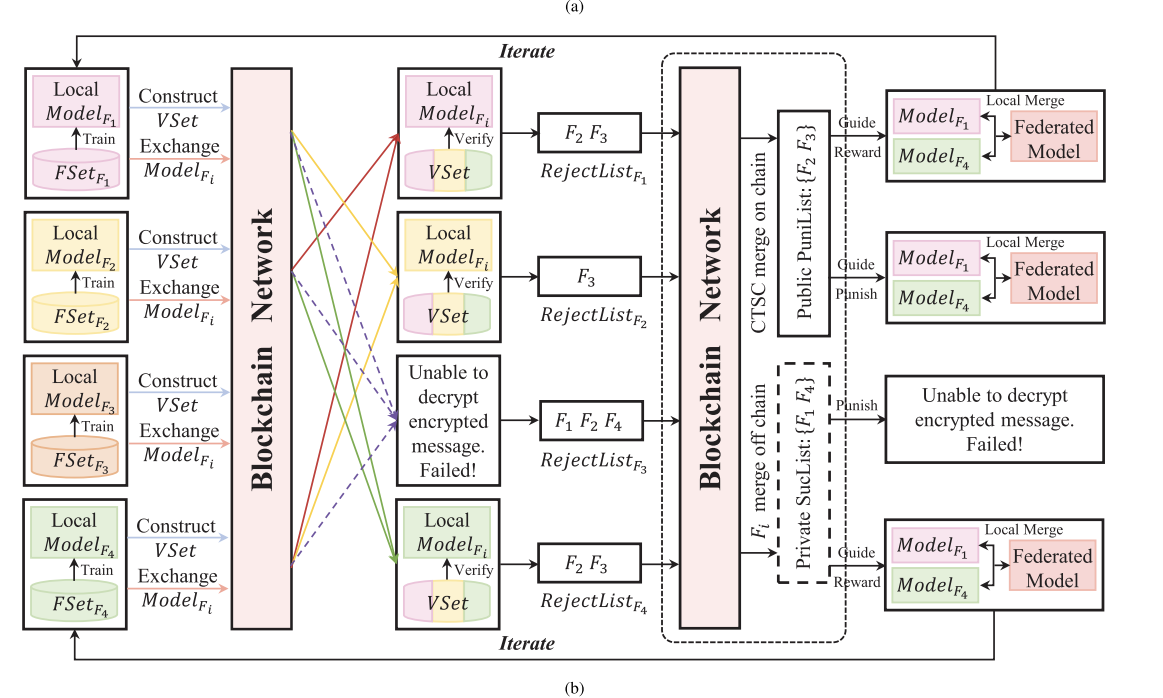
\includegraphics[scale=0.6]{figures/fig1-1.png}                    
        \end{column}
    \end{columns}
\end{frame}



  % スライド3: 罰則メカニズム
  \begin{frame}{罰則メカニズム}
    \begin{itemize}
      \item 各イテレーションで \(\mathrm{RejectList}_{F_i}\) の提出は 1 回に制限
      \item 全ての \(F_i\in \mathrm{ActiveList}_{FE}\) に
        「正しい \(\mathrm{len}(\mathrm{ActiveList}_{FE})\) を報告したが
        認識されていないメンバー」を監視し,\(\mathrm{RejectList}_{F_i}\) に追加する義務
      \item \(\mathrm{RejectList}_{F_i}\)/\(\mathrm{PuniList}\) に含まれるのが
        悪意メンバーか正直メンバーかは区別困難
      \item 最終的に \(\mathrm{PuniList}\) 登録者はデポジット全額没収
      \item 没収金 \(D_{\mathrm{Puni}}\) は正直メンバーに均等分配
    \end{itemize}
  \end{frame}
  
  % スライド4: CTSCの主要関数設計
  \begin{frame}{CTSCの主要な関数}
    \begin{itemize}
      \item 登録:正しい \(\mathrm{len}(\mathrm{ActiveList}_{FE})\) の報告
      \item \(\mathrm{VSet}_{F_i}\) 交換:イベント発火+モニタリング
      \item \(\mathrm{Model}_{F_i}\) 交換:同上
      \item \(\mathrm{RejectList}_{F_i}\) 報告:1アカウント1回に制限
      \item デポジット引き出し:イテレーション終了後1回のみ
      \item 全関数は所定の呼び出し可能時間内にのみ実行可能
      
      $|$- \(\mathrm{Model}_{FE}\) と資金の安全を保証
    \end{itemize}
  \end{frame}
  
  % スライド5: まとめ
  \begin{frame}{CTSCのまとめ}
    \begin{itemize}
      \item プライベートFL終了時,\(\mathrm{ActiveList}_{FE}\) メンバーは
        理想的な \(\mathrm{Model}_{FE}\) を取得
      \item 仮想通貨を通じて公平な報酬・罰則を実現
    \end{itemize}
  \end{frame}




    % \begin{frame}{実験1 数値シミュレーション}
    %     \begin{columns}
    %         \begin{column}[T]{.7\linewidth}
    %             \begin{itemize}
    %             \item 問題設定
    %             \begin{itemize}
    %                 \item ID 20,BS 3,RB 5
    %                 \item ID, BSは1kmの正方形空間にランダム配置
    %                 \item IDで生成されるデータの量: $\lambda_{i} = 100|1000$  Kbps
    %                 \item 学習時間の$T$における総量 50000 データ
    %                 \item ラベル数は10
    %                 \item 各IDのラベル分布$p_i (C)$はランダム
    %             \end{itemize}
    %             \item 生成データ量を変えて実験
    %             \item 式17の$\beta$依存性も見た
    %             \item データの量と分布を確認
    %             \item 最適化は4,8の制約に従う
    %             \end{itemize}          
    %         \end{column}
    %         \begin{column}[T]{.5\linewidth}
    %             \begin{center}
    %             % \includegraphics[scale=0.4]{figures/eq4.png}
    %             % \includegraphics[scale=0.4]{figures/eq8.png}
    %             \end{center}
    %         \end{column}
    %     \end{columns}
    % \end{frame}


    % \begin{frame}{実験1 数値シミュレーション}
    %     \begin{columns}
    %         \begin{column}[T]{.7\linewidth}
    %             \begin{itemize}
    %             \item ナイーブ法
    %                 \begin{itemize}
    %                     \item IDはランダムに配置
    %                     \item 最も近いBSに接続
    %                 \end{itemize}
    %             \end{itemize}          
    %         \end{column}
    %         \begin{column}[T]{.5\linewidth}
    %         \end{column}
    %     \end{columns}
    % \end{frame}


    % \begin{frame}{実験1の結果}
    %     \begin{columns}
    %         \begin{column}[T]{.5\linewidth}
    %             \begin{itemize}
    %             \item fig2の見方
    %                 \begin{itemize}
    %                     \item 星がBS
    %                     \item 点がID
    %                     \item 同じ色のBSに接続
    %                     \item 黒は未接続
    %                 \end{itemize}
    %             \end{itemize}    
    %         \end{column}
    %         \begin{column}[T]{.5\linewidth}
    %             \begin{center}
    %                 % \includegraphics[scale=0.3]{figures/fig-2.png}                    
    %             \end{center}
    %             \end{column}
    %     \end{columns}
    % \end{frame}

    % \begin{frame}{実験1の結果}
    %     \begin{columns}
    %         \begin{column}[T]{.6\linewidth}
    %             \begin{itemize}
    %             \item 図a,bの比較
    %                 \begin{itemize}
    %                     \item データ生成量の多寡
    %                     \item aは生成量小
    %                         \begin{itemize}
    %                             \item 制約8での送信先の縛りが緩い
    %                         \end{itemize}   
    %                     \item bは生成量大
    %                         \begin{itemize}
    %                             \item 扱うデータ量が増大
    %                             \item 制約がより厳しくなる
    %                             \item 近いBSに送信することが多い
    %                         \end{itemize}
    %                     \end{itemize}
    %             \item 提案手法とナイーブの比較
    %                 \begin{itemize}
    %                     \item 提案手法はBSに接続したIDの総量が多い
    %                     \item 利用したデータの数が多い
    %                     \item KL(p(c)¦pj (c))が小さい?
    %                 \end{itemize}
    %             \end{itemize}    
    %         \end{column}
    %         \begin{column}[T]{.5\linewidth}
    %             \begin{center}
    %                 % \includegraphics[scale=0.3]{figures/fig-2.png}                    
    %             \end{center}
    %             \end{column}
    %     \end{columns}
    % \end{frame}



    \section{4. 知見}
    \begin{frame}{得られた結果,知見}
        \begin{columns}
            \begin{column}{.8\linewidth}
                \begin{itemize}
                   \item 提案手法はコラボレーションコストを削減しつつ
                   \begin{itemize}
                    \item イーサリアム上での暗号通貨の支払額
                    \item 計算時間
                  \end{itemize}  
                  \item セキュリティやプライバシを担保
                \end{itemize}          
            \end{column}
        \end{columns}
    \end{frame}


    \section{5. 他}
    \begin{frame}{テーマについて}
        \begin{columns}
            \begin{column}{.8\linewidth}
                \begin{itemize}
                    \item 何かしら連合学習に使えそう
                    \item もし参考にするなら
                    \begin{itemize}
                        \item IoTデバイスのデータを集約するサーバを用意
                        \item 各サーバがbcのブロックとなり,FLに参加
                    \end{itemize}
                    \item 任意のノードを追加可能な設計にしたい
                    \item bcでモデルのバージョン管理などできないか?
                \item 次読むなら
                \item  Anton Wahrstatter et al. Openfl: A scalable and secure decentralized federated learning system on the ethereum
                blockchain. Internet of Things, 26:101174, 2024.
            \end{itemize}
        \end{column}
        \end{columns}
    \end{frame}

    \begin{frame}{分かっていない/気になる点}
        \begin{columns}
            \begin{column}{.8\linewidth}
                \begin{itemize}
                    \item イーサリアムとIPFSをどう使い分けているか
                    \begin{itemize}
                        \item 現状の認識
                        \begin{itemize}
                            \item 前者がインセンティブや識別に利用?
                            \item 後者がファイル共有に強いらしいので,モデル交換?
                        \end{itemize}
                    \end{itemize}
                    \item セキュリティとプライバシがどれくらい良いか
                    \begin{itemize}
                        \item 類似手法と比較したい
                        \item そもそもbcを使わないFLとも比較したい
                        \item いまいち効果がピンときていない
                        \item 何かしら追試を行いたい
                    \end{itemize}
                    \item 台帳上に保管されるデータはどれ?
                    \begin{itemize}
                        \item モデルのパスくらい?
                    \end{itemize}
                \end{itemize}          
            \end{column}
        \end{columns}
    \end{frame}

    \begin{frame}{分かっていない/気になる点}
        \begin{columns}
            \begin{column}{.8\linewidth}
                \begin{itemize}
                    \item オフチェーンとオンチェーンとは何か
                    \begin{itemize}
                        \item 前者が通常のFL
                        \item 後者がbc上のFL?
                        \item bc上のFLに参加できない $>$ ローカルで完結,という文脈?
                    \end{itemize}
                    \item 結局どのように学習しているか   
                    \begin{itemize}
                        \item プライバシとセキュリティ担保の取り組みは一通り見た
                        \item P2Pネットワーク上でどのようにモデルを交換する?
                        \item 今の認識
                        \begin{itemize}
                            \item 相互に信頼したリスト上の相手に逐次問い合わせ,交換
                        \item 最終的に信頼されたノードのみ含まれるグローバルモデルが完成
                        \end{itemize}
                    \end{itemize}
                \end{itemize}          
            \end{column}
        \end{columns}
    \end{frame}

\end{document}